\section{Visualization = Graphing + Fitting + Graphing}\label{sec:intro-visualize}
\epigraph{Look here, upon this picture, and on this.}{Shakespeare, Hamlet}

Statistical summaries, hypothesis tests, and the numerical parameters
derived in fitted models are designed to capture a particular feature of the
data.  An analysis of the data from \tabref{tab:berk220}, for example,
shows that 44.5\% of male applicants were admitted, compared to
30.4\% of female applicants, giving a Pearson chi-square of 92.2
with 1 degree of freedom
for association between admission and gender ($p < 0.001$).
Expressed in terms of the odds ratio, males were apparently
1.84 times as likely
to be admitted as females, with 99\% confidence bounds
1.562--2.170.
Each of these numbers expresses some part of the relationship between
gender and admission in the Berkeley data.

Numerical summaries, even for such a small \Dset\ as this,
are designed to compress the information in the data.
In contrast, the visualization approach to data analysis is designed
to 
\begin{seriate}
\item expose information and structure in the data,
\item supplement the information available from numerical summaries, and 
\item suggest more adequate models.
\end{seriate}
In general, the visualization approach seeks to serve the needs of
both summarization and exposure.

This approach recognizes that both data analysis and graphing are
iterative processes.
We should not expect that any one model captures all features of the
data any more than we should expect that a single graph shows all that
may be seen.  In most cases, our initial steps should include some
graphical display guided by understanding of the subject matter
of the data.
What we learn from a graph may then help suggest features of the data
to be incorporated into a fitted model.
A desire to ensure that the fitted model is an adequate summary
may then lead to additional graphs.

\begin{Example}[lifeboat0]{Lifeboats on the \emph{Titanic}}
One example is shown in \figref{fig:lifeboat}, described in more
detail in \exref{ex:lifeboat1}.
The left panel shows a trilinear plot of the composition of 
lifeboats on the \emph{Titanic}.
Each point in the plot shows the relative proportions of male
passengers
(identifying those with 10\% or more men), women and children and ``men of crew'' reported in each of the
18 lifeboats launched from the port and starboard sides of that
ill-fated vessel.
Trilinear plots are described in \secref{sec:twoway-trilinear},
but essentially, points near the top apex represent boats
nearly all filled with women and children.
%% two subfig side-by-side
\begin{figure}[htb]
 \begin{minipage}[c]{.49\linewidth}
  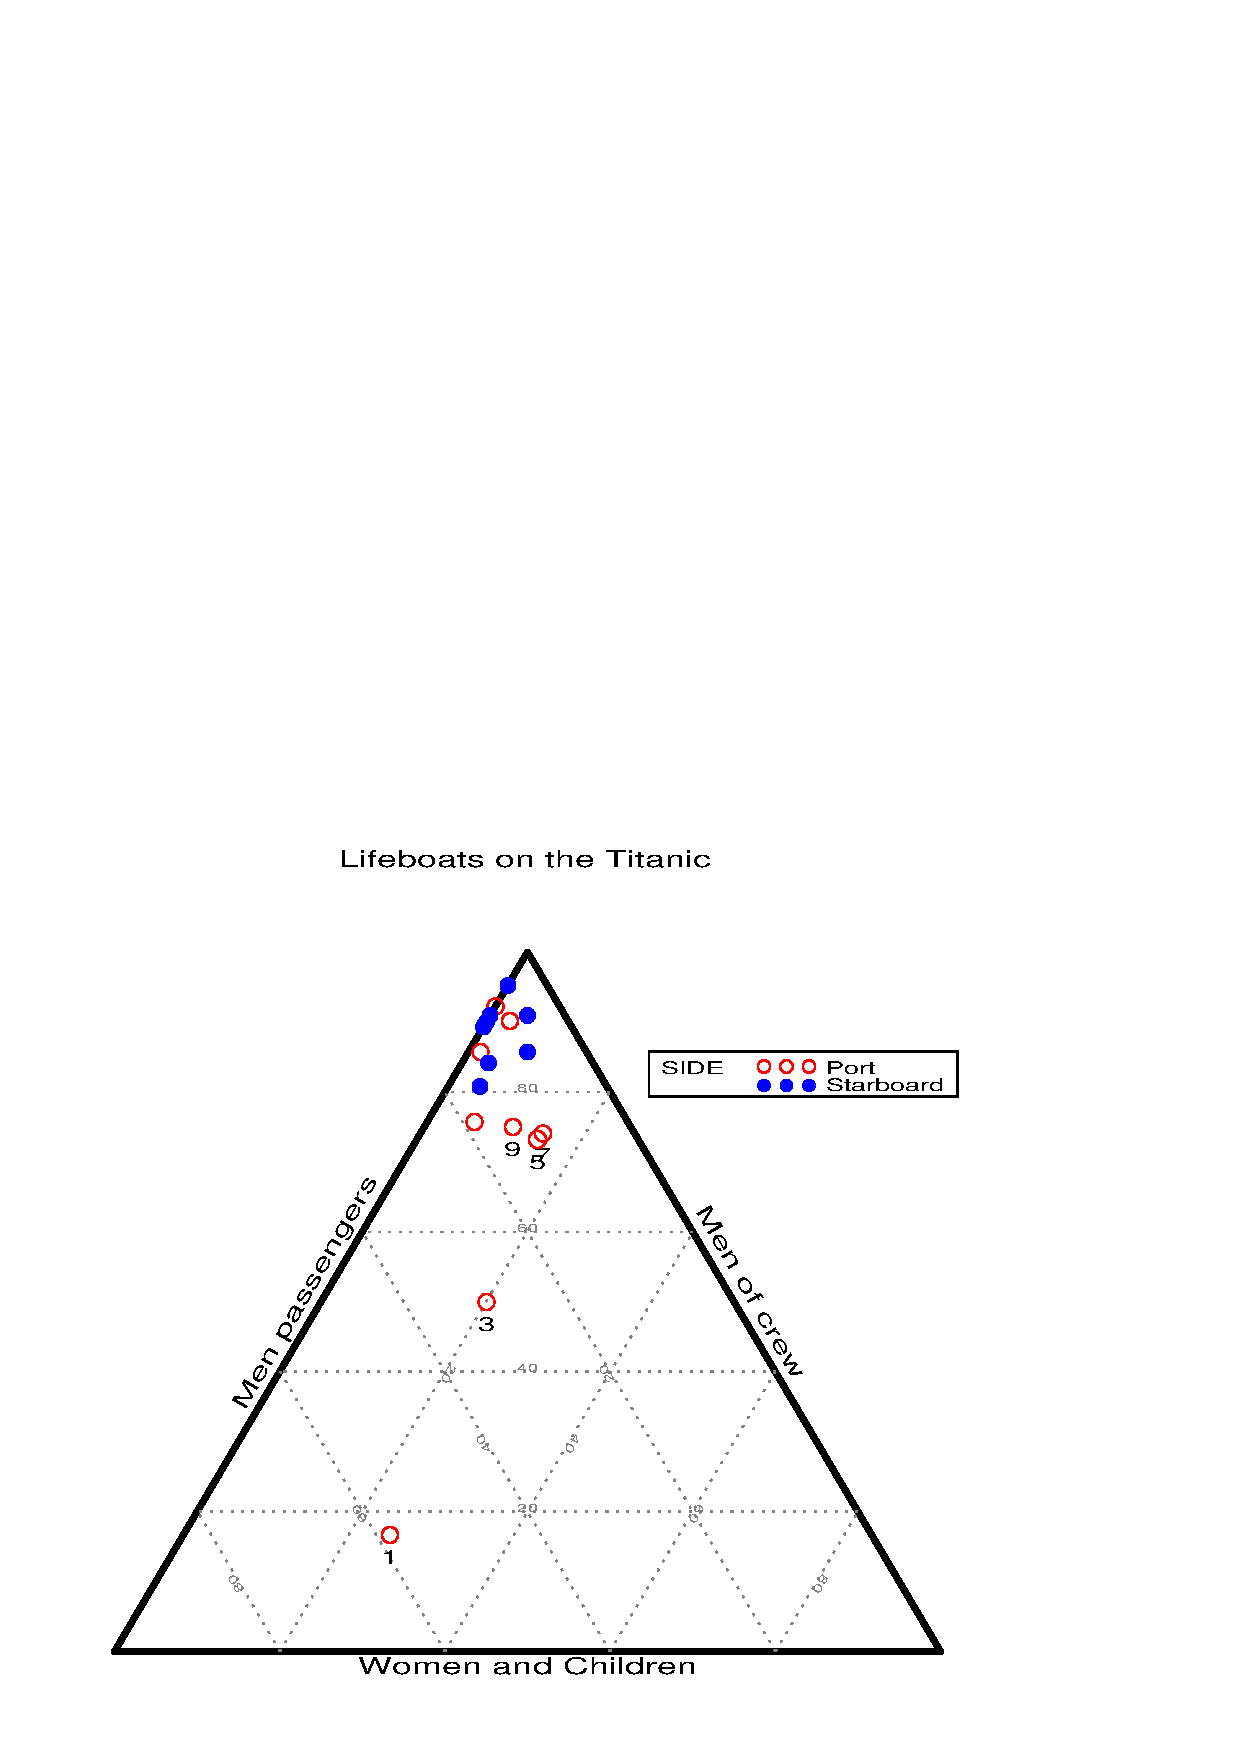
\includegraphics[width=1\linewidth,clip]{ch3/fig/lifeboat1}
 \end{minipage}%
 \hfill
 \begin{minipage}[c]{.49\linewidth}
  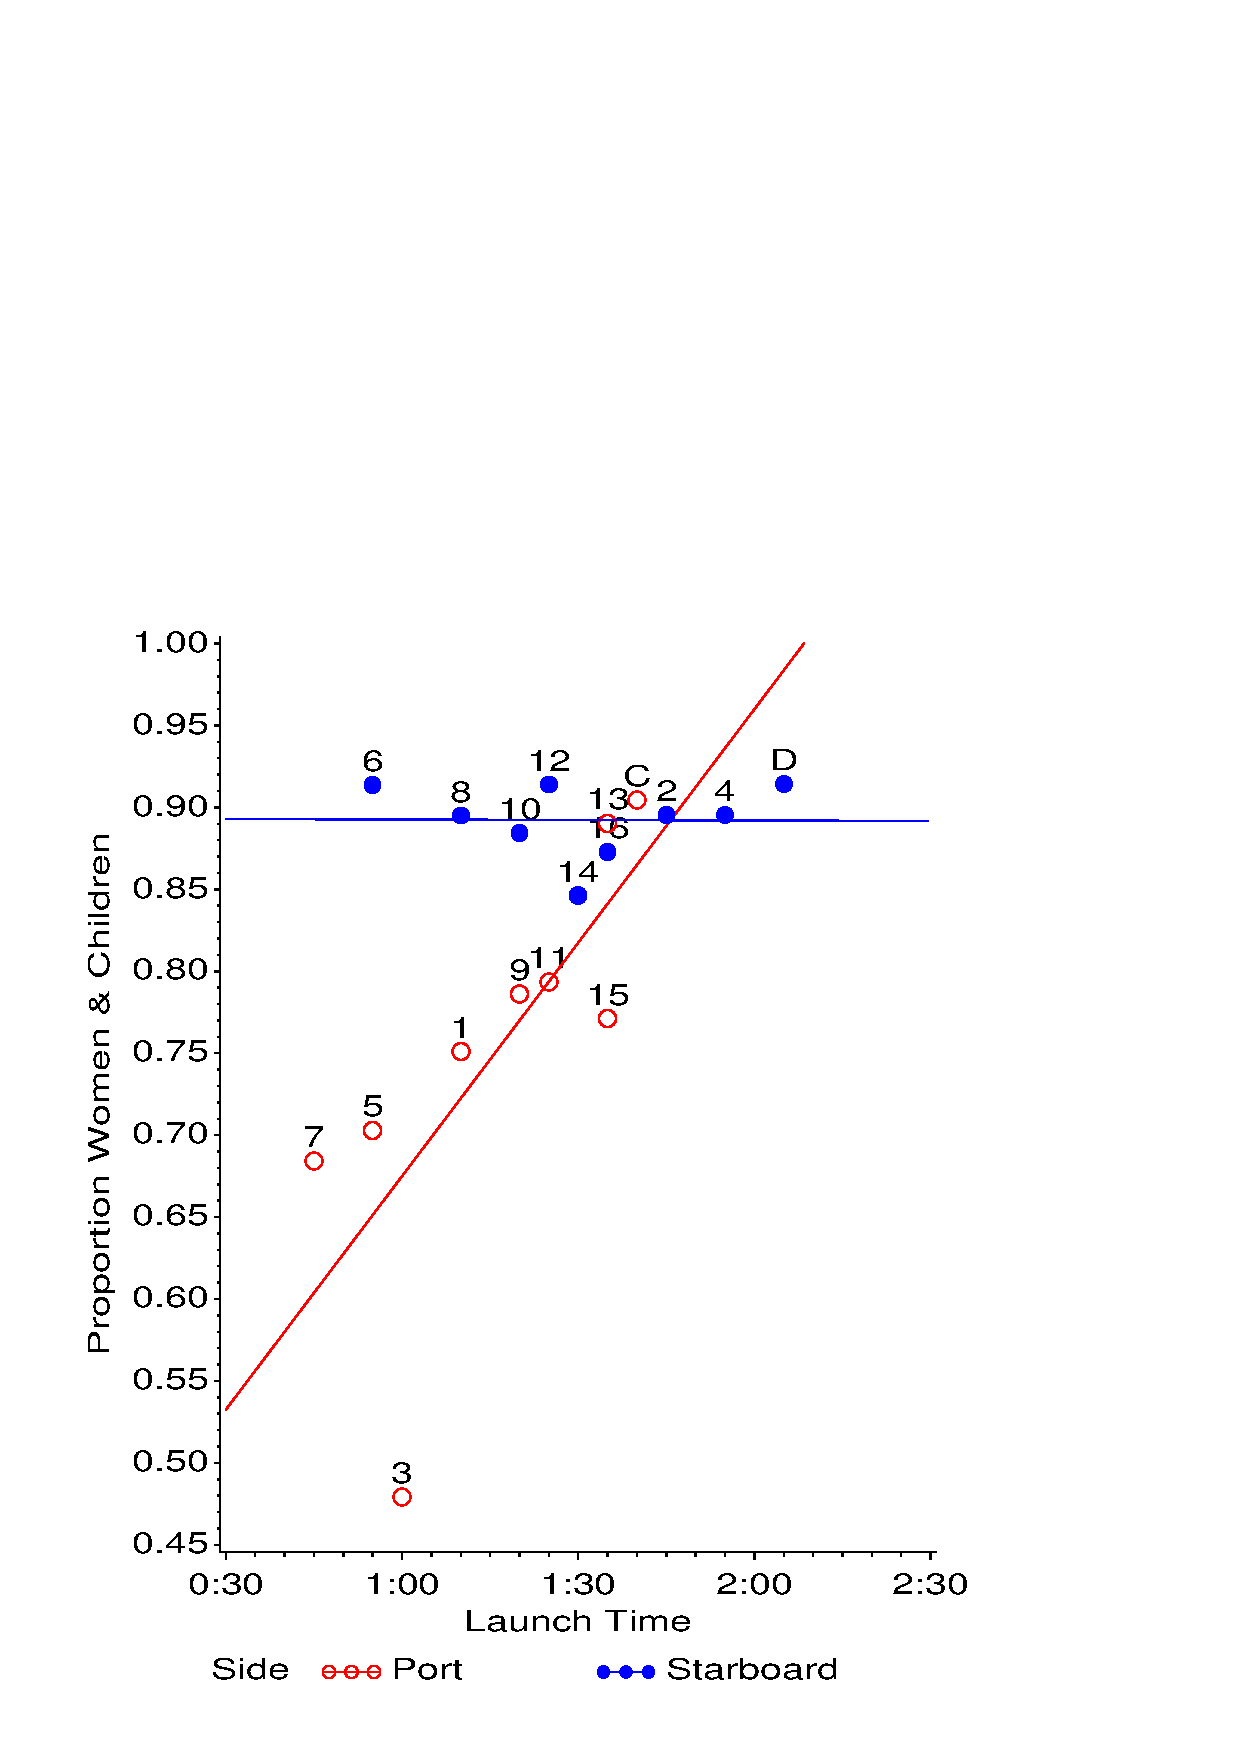
\includegraphics[width=1\linewidth,clip]{ch1/fig/lifeboat3}
 \end{minipage}
 \caption[Two graphical displays for \emph{Titanic} lifeboat data]{Two graphical displays for \emph{Titanic} lifeboat data. Left: trilinear plot, right: logistic regression.}\label{fig:lifeboat}
\end{figure}

That graph suggested that the procedures for loading the lifeboats
might have differed for the port and starboard side of the ship.
We were led to fit a logistic regression model predicting the
proportion of women and children loaded over time, with separate
slopes and intercepts for the port and starboard sides.
The right panel of \figref{fig:lifeboat} shows predicted proportions
from this model, with simple linear regression lines for the
two sides.  Even without further details about the data or
the analysis, the graph shows clearly that passengers on the two
sides of the \emph{Titanic} were subject to different regimes
for loading the lifeboats.
\end{Example}

This interplay between graphing and fitting may be expressed as
\begin{equation*}
\textrm{Visualization} = \textrm{Graphing} + \textrm{Fitting} + \textrm{Graphing} + \cdots
\comma
\end{equation*}
where the $\cdots$ remind us that there are often additional steps.

Sometimes a visualization is sufficiently strong (as, perhaps in
\figref{fig:glogist00} or the right panel of \figref{fig:lifeboat}),
that hypothesis tests and model parameters
serve an ancillary role in understanding the effects in the data. 
$p$-values are useful in the conventions of scientific communication,
but perhaps less convincing evidence than a graph whose conclusions hit you
between the eyes.

In other cases, graphing serves as a supporting member of the data-analytic
cast.  Model-based methods rely on assumptions about the data.
Diagnostic plots for logistic regression (\secref{sec:logist-infl})
and \loglin\ models (\secref{sec:loglin-infl})
may provide comfort that the assumptions on which these inferences
depend are reasonable for the data at hand, or suggest that some modification
of the model would help us rest more easily.

In any event, it is well to remember that data analysis requires both
summarization and exposure, and the needs of both are served by the
combination of graphing and fitting.

\subsection{Static vs.\ dynamic graphics}
\ix{graphics!static vs.\ dynamic|(}
The confines of a book and of the software that we describe here for
visualizing categorical data limit this presentation to static displays,
produced by SAS programs.  Many of these static graphics are made
considerably easier to use and more flexible by a number of SAS macros
illustrated in the following chapters and described in Appendix~\ref{ch:macros}.

The most productive use of these methods will require the addition of
two aspects of interactive graphics, presently being developed
by the author \citep{Friendly:96}
and by others \citep{TheusLauer:99,Young:94}.
\begin{itemize}
\item The first aspect relates to interactive methods for choosing variables,
parameters, and options for analysis and graphical displays.  The 
development tools for this form of interactivity are provided in \AF\
and most of the macro programs described here may be easily wrapped
in an interactive front-end.

\item A second aspect of dynamic graphics is related to the ability to interact
with multiple, linked  views of a \Dset, so that, for example,
selecting a subset of cases in one view highlights them in all other
views.  \INSIGHT\
is a prototype for this type of interaction in the SAS System.

\end{itemize}

We look forward to the development of more interactive methods and the
extension of multiple, linked data views for
categorical data with the SAS System.  Nevertheless, we need to understand
the various forms of graphic displays which are particularly useful
for discrete data before learning how to
employ them interactively.
\ix{graphics!static vs.\ dynamic|)}
